The knowledge of the nuclide chart far from the stabilty valley is one of the
fundamental topics for the nuclear structure studies, as it could hopefully
lead to the comprehension of the nuclear force, which is responsible both for
the abundance of stable nuclei and for weakly bound systems.
Nuclei can be formed in multiple diffrent combinations of protons and neutrons.
However, because of the fundamental forces and symmetries of Nature, not all
combinantions are stable and bound.

\bigbreak

The nuclear landscape show more than $3000$ of nuclei that are expected to be
bound by the strong force. Among these, less than $300$ are stable, while the
others are bound against the emission of protons and neutrons, or against the
$\beta$-decay, in which a proton decays into a neutron (or vice versa). Some
of the unstable nuclei are long-lived and found on Earth, some are produced
experimentally while other thousands, far from stabiity, are still undetected.
Consequently, from the multitude of nuclei that may exist and that could have
been formed i.e.\ in violent stellar explosions, only a very limited number
have been studied.

\bigbreak

\begin{figure}[h]
  \centering
  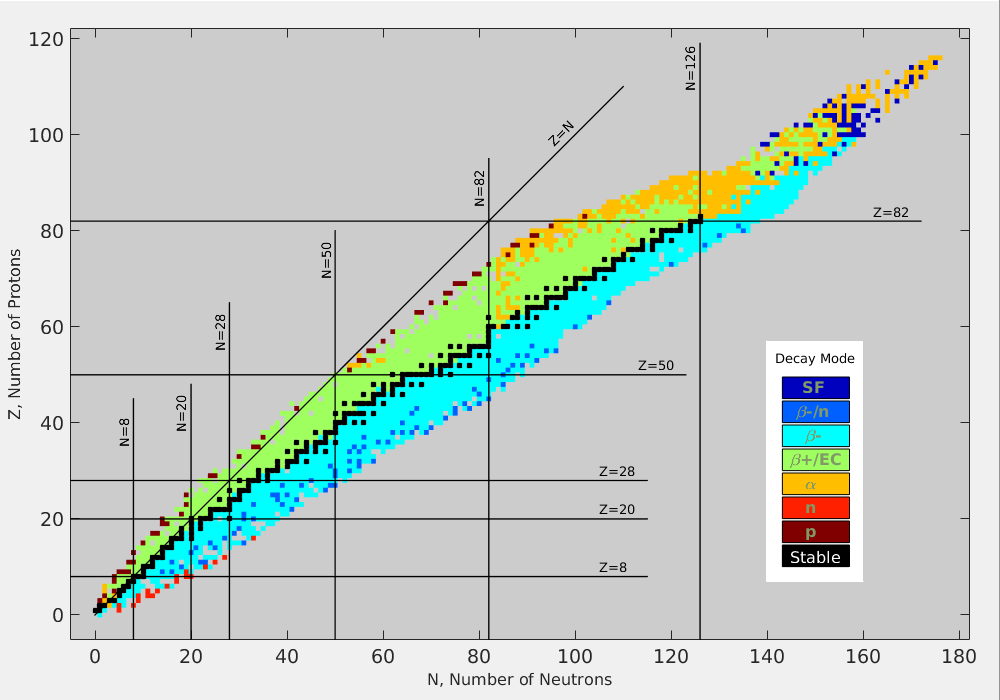
\includegraphics[scale=.35]{img/DecayModeNuDat2.png}
  \caption{The nuclide landscape}
  \label{nucl}
\end{figure}

\bigbreak

In particular, the neutron-rich light isotopes of \ce{Be}, \ce{C}, \ce{O} and
\ce{Ne} offer an extremely fertile ground for nuclear structure studies far
from stabilty region. On one hand, they may serve as examples of nuclear
clustering: for instance, in \ce{^12 C} many states have a well-established
$\alpha$-cluster structure. On the other hand, they exhibit features of
shell-model nuclei in which the impact of the continuum on the shell structure
has to be considered. This characteristics is clearly visible in \ce{^19 O},
in which a comprehensive analysis of the known excitations provides evidence
for states with single-particle structure and states which have strong
$\alpha$-clustering and form rotational bands.

\bigbreak

Description of excitations of the first type involve the standard nuclear
Shell Model (SM), which is an a priori approach; here, the degrees of freedom
are the valence protons and neutrons moving in specific shells – this model
cannot predict cluster states.
The second group of states can be treated with cluster models, which, in turn,
are a posteriori approaches that assume effective building blocks (clusters).
Both these approaches present, however, rather disjointed and not fully
consistent physical descriptions as they assume the nucleus to be a closed
quantum system that is completely isolated from the subspace of scattering and
decay channels. It is clear that a comprehensive understanding of low-energy
excitations in neutron-rich oxygen isotopes cannot emerge from such a picture.

\bigbreak

A significant step forward in creating the link between the SM approach and
the cluster approach to the structure of light nuclei was recently
made~\cite{oko:cluster}~\cite{oko:origin}.
It was showed that the mixing of SM eigenstates, induced by the external
coupling to the decay channel(s), profoundly impacts the nature of SM
eigenstates lying near particle-decay thresholds. 
It was concluded that the mixing of SM eigenstates (with the same quantum
numbers) via the continuum explains:

\begin{itemize}
\item the emergence of clustering leading to the appearance of
collective/cluster states located near the corresponding particle decay
thresholds
\item a gradual disappearance of charged-particle clustering in heavier nuclei
\end{itemize}

The $\alpha$-cluster states, being the best manifestation of the near-threshold
clustering phenomenon, cannot, however, be calculated with the SMEC Model
approach yet. The other class of near-particle-decay threshold states are
states lying close to the nucleon-decay thresholds - they are also
commonly observed in light nuclei. Here, the degree of collectivization can be
predicted by the SMEC Model, but the clear comparison with experiment has not
yet been done. 

\bigbreak

In this context, the measurement of electromagnetic decay from unbound
near-threshold states in neutron-rich systems, which could prove the predicted
near-threshold collectivization phenomenon by the observation of the increase
of electromagnetic transitions probability, would represent a breakthrough.
At present, such information is almost totally missing, as a consequence of
very low  $\gamma$-decay branchings, of the order of $10^{-3}$-$10^{-4}$ and
even lower. The studies call then for the use of very selective reaction
mechanisms and $\gamma$ spectrometers, in order to enhance the sensitivity to
the population of unbound states and their electromagnetic decays.